%
%  untitled
%
%  Created by Parham Aram on 2010-07-14.
%  Copyright (c) 2010 . All rights reserved.
%
\documentclass[]{article}

% Setup for fullpage use
\usepackage{fullpage}

\usepackage[pdftex]{graphicx}


% More symbols
\usepackage{amsmath}
\usepackage{amssymb}

\usepackage[usenames,dvipsnames]{color}
\newcommand{\dean}[1]{\textcolor{red}{#1}}
\newcommand{\parham}[1]{\textcolor{blue}{#1}}

\begin{document}


\renewcommand{\theequation}{S1.\arabic{equation}}


\subsection*{Estimation of Connectivity Kernel Support}
The support of the connectivity kernel can be inferred using spatial correlation analysis. The method presented in this paper is based on a similar published method, where the kernel support was estimated using correlation analysis for a linear system described by an IDE~\cite{Scerri2009}. To demonstrate the method for the neural field model we assume the sensors are infinitesimally close (continuous observation). The spatial cross-correlation function between consecutive observations is defined as 
\begin{align}
	R_{y_{t},y_{t+1}}(\boldsymbol{\tau}) &= \mathbf{E}\left[ y_{t}\left(\mathbf{r}\right) y_{t+1}\left(\mathbf{r}+\boldsymbol{\tau}\right) \right] \\
	&= \mathbf{E}\left[\left(\left(m\ast v_t\right)\left(\mathbf{r}\right) + \boldsymbol{\varepsilon}_t\left(\mathbf{r}\right) \right) \times \left(\left( m \ast v_{t+1}\right)\left(\mathbf{r}+\boldsymbol{\tau}\right)+ \boldsymbol{\varepsilon}_{t+1}\left(\mathbf{r}+\boldsymbol{\tau}\right)\right) \right], \label{eq:ObsXCorr}
\end{align}

where $\mathbf{E}[\cdot]$ is the expected value. Since the observation noise is zero mean, temporally white and independent of the field, equation~\ref{eq:ObsXCorr} reduces to
\begin{equation}
	R_{y_{t},y_{t+1}}(\boldsymbol{\tau}) = \mathbf{E}\left[ \left(m \ast v_t\right)\left(\mathbf{r}\right) \times \left(m \ast v_{t+1}\right)\left(\mathbf{r}+\boldsymbol{\tau}\right)\right].
\end{equation}
Substituting in equation~\ref{DiscreteTimeModel}  for $v_{t+1}\left(\mathbf{r}\right)$, the cross-correlation function is
\begin{align}
	R_{y_{t},y_{t+1}}(\boldsymbol{\tau}) &= \mathbf{E}\left[ \left(m \ast v_t \right)\left(\mathbf{r}\right) \times m\left(\mathbf{r}+\boldsymbol{\tau}\right) \ast \left( \xi v_t\left(\mathbf{r}+\boldsymbol{\tau}\right) + T_s w\left(\mathbf{r}+\boldsymbol{\tau}\right) \ast f\left(v_t\left(\mathbf{r}+\boldsymbol{\tau}\right)\right) + e_t\left(\mathbf{r}+\boldsymbol{\tau}\right)\right) \right] \nonumber \\	
	 &= \xi \mathbf{E}\left[ \left(m \ast v_t \right)\left(\mathbf{r}\right) \times \left(m \ast v_t\right)\left(\mathbf{r}+\boldsymbol{\tau}\right)\right] \nonumber \\
	&+ T_s\mathbf{E}\left[\left(m \ast v_t \right)\left(\mathbf{r}\right) \times \left(m \ast w \right)\left(\mathbf{r}+\boldsymbol{\tau}\right) \ast f\left(v_t\left(\mathbf{r}+\boldsymbol{\tau}\right)\right) \right] \nonumber \\
	&+ \mathbf{E}\left[ \left(m \ast v_t \right)\left(\mathbf{r}\right)  \times \left(m \ast e_t\right)\left(\mathbf{r}+\boldsymbol{\tau}\right)\right] \nonumber \\
	&= R_1(\boldsymbol{\tau}) + R_2(\boldsymbol{\tau}) + R_3(\boldsymbol{\tau}).\label{eq:spatialxcorr} 
\end{align}
For simplicity we use $z_{t}\left(\mathbf{r}\right)$ to denote noise free observations, i.e.,
\begin{align}
z_{t}\left(\mathbf r\right)&=\left(m\ast v_{t}\right)\left(\mathbf{r}\right). 
\end{align}
The first term, $R_1(\boldsymbol{\tau})$, can be simplified to
\begin{align}
	R_1(\boldsymbol{\tau}) &= \xi \mathbf{E}\left[z_{t}\left(\mathbf r\right)  z_{t}\left(\mathbf{r}+\boldsymbol{\tau}\right) \right] \\
	&= \xi\left( R_{y_{t},y_{t}}(\boldsymbol{\tau}) - \sigma_{\varepsilon}^2\delta_K\left(\boldsymbol{\tau}\right) \right). \label{eq:R1}
\end{align}
% The second term
% \begin{equation}
% 	R_2(\boldsymbol{\tau}) = T_s\mathbf{E}\left[ m\left(\mathbf{r}\right) \ast v_t\left(\mathbf{r}\right) \times m\left(\mathbf{r}+\boldsymbol{\tau}\right) \ast w\left(\mathbf{r}+\boldsymbol{\tau}\right) \ast f\left(v_t\left(\mathbf{r}+\boldsymbol{\tau}\right)\right) \right]
% \end{equation}
Now we assume that the sigmoid activation function, $f(\cdot)$, can be approximated by the piecewise function
\begin{equation}
	\hat{f}(v_t(\mathbf{r}')) = \left\{ \begin{array}{ll}
		0, & v_t(\mathbf{r}') \le v_1 \\
		\varsigma v_t(\mathbf{r}'), &  v_1 < v_t(\mathbf{r}') < v_2 \\
		1, & v_t(\mathbf{r}') \ge v_2 \\ 
		\end{array}\right.
\end{equation}
Furthermore, we assume the field is in the linear region of the piecewise function for the majority of the time giving
\begin{equation}
	R_2(\boldsymbol{\tau}) \approx T_s \varsigma \mathbf{E}\left[ z_{t}\left(\mathbf{r}\right)\times \left(z_{t} \ast w\right)\left(\mathbf{r}+\boldsymbol{\tau}\right)\right].
\end{equation}
$R_2(\boldsymbol{\tau})$ can be written as
\begin{align}
	R_2(\boldsymbol{\tau}) &\approx T_s \varsigma \mathbf{E}\left[ z_{t}\left(\mathbf{r}\right)  \int_{\Omega}z_{t}\left(\mathbf{r'}\right) w\left(\mathbf{r}+\boldsymbol{\tau}-\mathbf{r'}\right) d\mathbf{r'} \right] \\
	&= T_s \varsigma \mathbf{E}\left[  \int_{\Omega}z_{t}\left(\mathbf{r}\right)z_{t}\left(\mathbf{r'}\right) w\left(\mathbf{r}+\boldsymbol{\tau}-\mathbf{r'}\right) d\mathbf{r'} \right] \\
	&= T_s \varsigma \mathbf{E}\left[  \int_{\Omega}z_{t}\left(\mathbf{r}\right)z_{t}\left(\mathbf{r}+\mathbf{r'}\right) w\left(\boldsymbol{\tau}-\mathbf{r'}\right) d\mathbf{r'} \right] \\
	&= T_s \varsigma   \int_{\Omega}\mathbf{E}\left[z_{t}\left(\mathbf{r}\right)z_{t}\left(\mathbf{r}+\mathbf{r'}\right) \right] w\left(\boldsymbol{\tau}-\mathbf{r}'\right) d\mathbf{r'}  \\
	&= \frac{T_s \varsigma}{\xi} \int_{\Omega} R_1(\mathbf{r'}) w\left(\boldsymbol{\tau}-\mathbf{r}'\right) d\mathbf{r'}  \\
	&= \frac{T_s \varsigma}{\xi} \left(R_1 \ast w\right)\left(\boldsymbol{\tau}\right)\\
\end{align}
The last term on the right hand side of equation~\ref{eq:spatialxcorr} is
\begin{equation}
	R_3(\boldsymbol{\tau}) = 0,
\end{equation}
since the disturbance added to the field at time $t$ and assumed to be uncorrelated to the field at time $t$. Therefore 
\begin{equation}
	R_{y_{t},y_{t+1}}(\boldsymbol{\tau}) - R_1(\boldsymbol{\tau}) \approx \frac{T_s \varsigma}{\xi} \left(R_1 \ast w\right)\left(\boldsymbol{\tau}\right).
\end{equation}
Now, by taking the Fourier transform we get
\begin{equation}
	\mathcal{F}\left\{R_{y_{t},y_{t+1}}(\boldsymbol{\tau})\right\} - \mathcal{F}\left\{R_1(\boldsymbol{\tau})\right\} \approx \frac{T_s \varsigma}{\xi} \mathcal{F}\left\{R_1(\boldsymbol{\tau})\right\} \mathcal{F}\left\{ w\left(\boldsymbol{\tau}\right)\right\}.
\end{equation}
This simplifies to
\begin{equation}
	\frac{\xi}{T_s \varsigma} \left(\frac{\mathcal{F}\left\{R_{y_{t},y_{t+1}}(\boldsymbol{\tau})\right\}}{\mathcal{F}\left\{R_1(\boldsymbol{\tau})\right\}} - 1\right) \approx  \mathcal{F}\left\{ w\left(\boldsymbol{\tau}\right)\right\}.
\end{equation}
Now substituting back in equation~\ref{eq:R1}, we can write

\begin{align}
	\mathcal{F}\left\{ w\left(\boldsymbol{\tau}\right)\right\} &\approx \frac{\xi}{T_s \varsigma} \left(\frac{\mathcal{F}\left\{R_{y_{t},y_{t+1}}(\boldsymbol{\tau})\right\}}{\mathcal{F}\left\{\xi\left( R_{y_{t},y_{t}}(\boldsymbol{\tau}) - \sigma_{\varepsilon}^2\delta_K\left(\boldsymbol{\tau}\right) \right)\right\}} - 1\right)  \\
	&= \frac{1}{T_s \varsigma} \left(\frac{\mathcal{F}\left\{R_{y_{t},y_{t+1}}(\boldsymbol{\tau})\right\}}{\mathcal{F}\left\{ R_{y_{t},y_{t}}(\boldsymbol{\tau})\right\} - \sigma_{\varepsilon}^2 } - \xi\right) \\
	&= \frac{1}{T_s \varsigma} \left(\frac{S_{y_{t},y_{t+1}}\left(\boldsymbol{\nu}\right)}{S_{y_{t},y_{t}}\left(\boldsymbol{\nu}\right) - \sigma_{\varepsilon}^2 } - \xi\right)
\end{align}

This equation states that the support of the kernel can be estimated given knowledge of $\sigma_\varepsilon^2$. The other parameters simply give an offset and scale the kernel. Furthermore, if we guess $\sigma_\varepsilon^2$ incorrectly, then the effect will only appear at $\boldsymbol{\tau}=0$. So if we assume local excitation, then we do not need to know $\sigma_\varepsilon^2$.


We can also write
\begin{equation}
	R_2(\boldsymbol{\tau}) \approx T_s \varsigma (R_{y_{t},y_{t}}(\boldsymbol{\tau}) - \sigma_{\varepsilon}^2\delta_K\left(\boldsymbol{\tau}\right)) \ast w(\boldsymbol{\tau})  
\end{equation}


\begin{align}
	R_2(\boldsymbol{\tau}) &\approx R_{y_{t},y_{t+1}}(\boldsymbol{\tau}) - R_1(\boldsymbol{\tau}) \\
	T_s \varsigma (R_{y_{t},y_{t}}(\boldsymbol{\tau}) - \sigma_{\varepsilon}^2\delta_K\left(\boldsymbol{\tau}\right)) \ast w\left(\boldsymbol{\tau}\right) &\approx R_{y_{t},y_{t+1}}(\boldsymbol{\tau}) - \xi\left( R_{y_{t},y_{t}}(\boldsymbol{\tau}) - \sigma_{\varepsilon}^2\delta_K\left(\boldsymbol{\tau}\right))  \right)
\end{align}
Take FFT of both sides
\begin{align}
	T_s \varsigma (S_{y_{t},y_{t}}\left(\boldsymbol{\nu}\right) - \sigma_{\varepsilon}^2) W\left(\boldsymbol{\nu}\right) &\approx S_{y_{t},y_{t+1}}\left(\boldsymbol{\nu}\right) - \xi (S_{y_{t},y_{t}}\left(\boldsymbol{\nu}\right) - \sigma_{\varepsilon}^2) \\
	W\left(\boldsymbol{\nu}\right) &\approx \frac{S_{y_{t},y_{t+1}}\left(\boldsymbol{\nu}\right) - \xi (S_{y_{t},y_{t}}\left(\boldsymbol{\nu}\right) - \sigma_{\varepsilon}^2)}{T_s \varsigma (S_{y_{t},y_{t}}\left(\boldsymbol{\nu}\right) - \sigma_{\varepsilon}^2)}
\end{align}

\begin{figure}[!ht]
\begin{center}
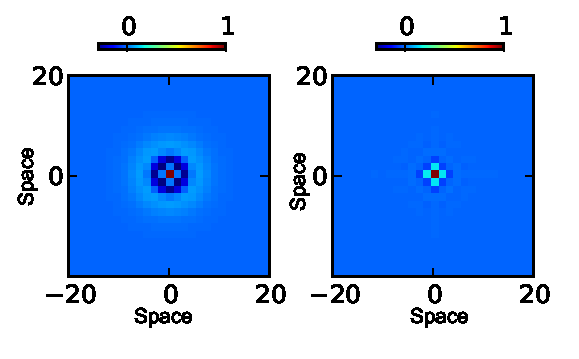
\includegraphics{./Figures/KernelWidthEstimation.pdf}
\end{center}
\caption{{\bf Estimation of Connectivity Kernel Support}. The kernel values are normalised. True  and estimated kernels are shown with solid and dotted lines respectively.}
\label{fig:KernelWidth}
\end{figure}

\begin{figure}[!ht]
\begin{center}
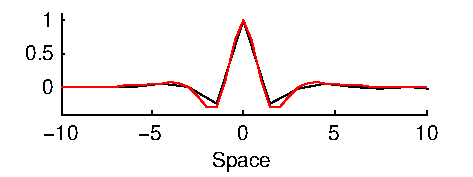
\includegraphics{./Figures/KernelWidthEstimation2.pdf}
\end{center}
\caption{{\bf Estimation of Connectivity Kernel Support}. The kernel values are normalised. True  and estimated kernels are shown with black and red lines respectively.}
\label{fig:KernelWidth2}
\end{figure}

\newpage
\subsection*{Estimation of Disturbance Support}
Given the knowledge of the sensors' spatial bandwidth, the support of the disturbance can be also inferred using spatial correlation analysis. Here we also assume continuous observation and the linear behaviour of the firing rate for majority of the time. The spatial auto-correlation function between observations at each time  is defined as 
\begin{align}
	R_{y_{t+1},y_{t+1}}(\boldsymbol{\tau}) &= \mathbf{E}\left[ y_{t+1}\left(\mathbf{r}\right) y_{t+1}\left(\mathbf{r}+\boldsymbol{\tau}\right) \right] \nonumber \\
	&= \mathbf{E}\left[\left(z_{t+1}\left(\mathbf r\right)  + \boldsymbol{\varepsilon}_{t+1}\left(\mathbf{r}\right) \right) \times \left(z_{t+1}\left(\mathbf{r}+\boldsymbol{\tau}\right)+ \boldsymbol{\varepsilon}_{t+1}\left(\mathbf{r}+\boldsymbol{\tau}\right)\right) \right] \nonumber \\
 &= \mathbf{E}\left[z_{t+1}\left(\mathbf r\right)  \times z_{t+1}\left(\mathbf{r}+\boldsymbol{\tau}\right) \right]+\sigma_{\epsilon}^2\delta_{K}\left(\boldsymbol\tau\right),\label{eq:ObsXCorrtplusone}
\end{align}
substituting for
\begin{align}
z_{t+1}\left(\mathbf r\right)&=\xi z_{t}\left(\mathbf r\right)+T_s\varsigma\left(z_t \ast w\right)\left(\mathbf r\right)+\left(m\ast e_t\right)\left(\mathbf r\right),\label{eq:zvariable}
\end{align}
in equation \ref{eq:ObsXCorrtplusone} yields
\begin{align}
	R_{y_{t+1},y_{t+1}}(\boldsymbol{\tau}) &=  \xi^2\mathbf{E}\left[ z_t\left(\mathbf r\right)z_t\left(\mathbf r+\boldsymbol \tau\right)\right] \nonumber \\
						&+\xi T_s\varsigma \ \mathbf{E}\left[z_t\left(\mathbf r\right)\left(z_t \ast w\right)\left(\mathbf r+\boldsymbol\tau\right)\right]\nonumber \\
						&+\xi T_s\varsigma \ \mathbf{E}\left[\left(z_t \ast w\right)\left(\mathbf r\right)z_t\left(\mathbf r+\boldsymbol\tau\right)\right]\nonumber \\
						&+T_s^2\varsigma^2 \ \mathbf{E}\left[\left(z_t \ast w\right)\left(\mathbf r\right)\left(z_t \ast w\right)\left(\mathbf r+\boldsymbol\tau\right)\right]\nonumber \\
						&+\mathbf{E}\left[\left(m \ast e_t\right)\left(\mathbf r\right)\left(m \ast e_t\right)\left(\mathbf r+\boldsymbol\tau\right)\right]+\sigma_{\epsilon}^2\delta_{K}\left(\boldsymbol\tau\right).\label{eq:AutocorrExpansion}
\end{align}
Equation \ref{eq:AutocorrExpansion} can be written in terms of $R_1\left(\boldsymbol\tau\right)$ and $R_2\left(\boldsymbol\tau\right)$ defined in equation~\ref{eq:spatialxcorr}
\begin{align}
R_{y_{t+1},y_{t+1}}(\boldsymbol{\tau}) &=\xi \left(R_1\left(\boldsymbol\tau\right)+ R_2\left(\boldsymbol\tau\right)+R_2\left(\boldsymbol-\tau\right)\right) \nonumber \\
&+\xi T_s \varsigma\left(w\ast R_2\right)\left(\boldsymbol\tau\right)+\left(m\ast m \ast \gamma\right)\left(\boldsymbol\tau\right)+\sigma_{\epsilon}^2\delta_{K}\left(\boldsymbol\tau\right),\label{eq:AutocorrIntermsofR}
\end{align}
 since $R_{y_{t},y_{t+1}}(\boldsymbol{\tau})=R_1\left(\boldsymbol\tau\right)+ R_2\left(\boldsymbol\tau\right)$, we can write
\begin{align}
R_{y_{t},y_{t}}(\boldsymbol{\tau}) &=\xi \left(R_{y_{t},y_{t+1}}(\boldsymbol{\tau})+R_2\left(\boldsymbol-\tau\right)\right) \nonumber \\
&+\xi T_s \varsigma\left(w\ast R_2\right)\left(\boldsymbol\tau\right)+\left(m\ast m \ast \gamma\right)\left(\boldsymbol\tau\right)+\sigma_{\epsilon}^2\delta_{K}\left(\boldsymbol\tau\right)
\end{align}
Note that we changed the time index as equation \ref{eq:AutocorrIntermsofR} is correct at all time. Now by taking the Fourier transform we get
\begin{align}
 \mathcal{F}\left\{\left(m\ast m\ast \gamma\right)\left(\boldsymbol\tau\right)\right\}&=S_{y_{t},y_{t}}\left(\boldsymbol\nu\right)-\xi S_{y_{t},y_{t+1}}\left(\boldsymbol\nu\right)-\xi \mathcal{F}\left\{R_2\left(-\boldsymbol\tau\right)\right\} \nonumber\\
&-\xi T_s \varsigma  \mathcal{F}\left\{w\left(\boldsymbol\tau\right)\right\}\mathcal{F}\left\{R_2\left(\boldsymbol\tau\right)\right\}-\sigma_{\epsilon}^2. \label{eq:SensorsConvgamma}
\end{align}
Fourier transforms of $R_2\left(\boldsymbol\tau\right)$ and its multiplication by  $w\left(\boldsymbol\tau\right)$ can be written in terms of $S_{y_{t},y_{t}}$ and $S_{y_{t},y_{t+1}}$
\begin{align}
 \mathcal{F}\left\{R_2\left(\boldsymbol\tau\right)\right\}=S_{y_{t},y_{t+1}}\left(\boldsymbol\nu\right)-\xi \left(S_{y_{t},y_{t}}\left(\boldsymbol\nu\right)-\sigma_{\epsilon}^2\right),
\end{align}
and
\begin{align}
 \mathcal{F}\left\{w\left(\boldsymbol\tau\right)\right\}\mathcal{F}\left\{R_2\left(\boldsymbol\tau\right)\right\}&=\frac{1}{T_s \varsigma}\left[\frac{S_{y_{t},y_{t+1}}^2\left(\boldsymbol\nu\right)}{S_{y_{t},y_{t}}\left(\boldsymbol\nu\right)-\sigma_{\epsilon}^2}-2\xi S_{y_{t},y_{t+1}}\left(\boldsymbol\nu\right)+\xi^2\left(S_{y_{t},y_{t}}\left(\boldsymbol\nu\right)-\sigma_{\epsilon}^2\right)\right].
\end{align}
Substituting in equation~\ref{eq:SensorsConvgamma} we get
\begin{align}
 \mathcal{F}\left\{\left(m\ast m\ast \gamma\right)\left(\boldsymbol\tau\right)\right\}&=S_{y_{t},y_{t}}\left(\boldsymbol\nu\right)-\xi S_{y_{t},y_{t+1}}\left(\boldsymbol\nu\right) \nonumber \\
&-\xi S_{y_{t},y_{t+1}}\left(-\boldsymbol\nu\right)-\xi^2 \left(S_{y_{t},y_{t}}\left(\boldsymbol\nu\right)-\sigma_{\epsilon}^2\right) \nonumber\\
&-\xi  \left[\frac{S_{y_{t},y_{t+1}}^2\left(\boldsymbol\nu\right)}{S_{y_{t},y_{t}}\left(\boldsymbol\nu\right)-\sigma_{\epsilon}^2}-2\xi S_{y_{t},y_{t+1}}\left(\boldsymbol\nu\right)+\xi^2\left(S_{y_{t},y_{t}}\left(\boldsymbol\nu\right)-\sigma_{\epsilon}^2\right)\right]-\sigma_{\epsilon}^2
\end{align}
Note that, the exact knowlege of $\sigma_{\epsilon}^2$ and $\xi$ are not required, since arbitrary values of these parameters do not affect the disturbance width significantly, however a good approximate of the sensor width is needed.
\begin{figure}[!ht]
\begin{center}
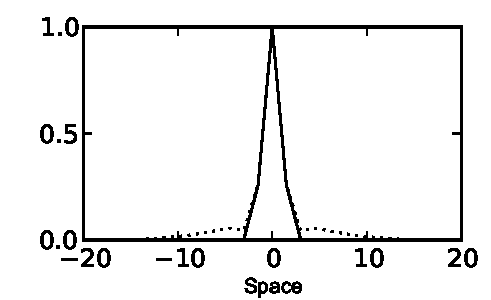
\includegraphics{./Figures/DisturbanceWidthEstimation.pdf}
\end{center}
\caption{{\bf Estimation of $\left(m\ast m \ast \gamma \right)\left(\boldsymbol \tau\right) $ width}. Values are normalised. True  and estimated values are shown with solid and dotted lines respectively.}
\label{fig:DisturbanceWidth}
\end{figure}
\bibliographystyle{plain}
\bibliography{}
\end{document}
